\documentclass[handout]{beamer} % sin pausas
%\documentclass{beamer} % con pausas
%\setbeamertemplate{background}[grid][step=8 ] % cuadriculado

\usetheme{CambridgeUS}


\usepackage{etex}
\usepackage{t1enc}
\usepackage[spanish,es-nodecimaldot]{babel}
\usepackage{latexsym}
\usepackage[utf8]{inputenc}
\usepackage{verbatim}
\usepackage{multicol}
\usepackage{amsgen,amsmath,amstext,amsbsy,amsopn,amsfonts,amssymb}
\usepackage{amsthm}
\usepackage{calc}         % From LaTeX distribution
\usepackage{graphicx}     % From LaTeX distribution
\usepackage{ifthen}
%\usepackage{makeidx}
\input{random.tex}        % From CTAN/macros/generic
\usepackage{subfigure} 
\usepackage{tikz}
\usepackage[customcolors]{hf-tikz}
\usetikzlibrary{arrows}
\usetikzlibrary{matrix}
\tikzset{
    every picture/.append style={
        execute at begin picture={\deactivatequoting},
        execute at end picture={\activatequoting}
    }
}
\usetikzlibrary{decorations.pathreplacing,angles,quotes}
\usetikzlibrary{shapes.geometric}
\usepackage{mathtools}
\usepackage{stackrel}
%\usepackage{enumerate}
\usepackage{enumitem}
\usepackage{tkz-graph}
\usepackage{polynom}
\polyset{%
    style=B,
    delims={(}{)},
    div=:
}
\renewcommand\labelitemi{$\circ$}
\setlist[enumerate]{label={(\arabic*)}}
\setbeamertemplate{itemize item}{$\circ$}
\setbeamertemplate{enumerate items}[default]
\definecolor{links}{HTML}{2A1B81}
\hypersetup{colorlinks,linkcolor=,urlcolor=links}


\newcommand{\Id}{\operatorname{Id}}
\newcommand{\img}{\operatorname{Im}}
\newcommand{\nuc}{\operatorname{Nu}}
\newcommand{\im}{\operatorname{Im}}
\renewcommand\nu{\operatorname{Nu}}
\newcommand{\la}{\langle}
\newcommand{\ra}{\rangle}
\renewcommand{\t}{{\operatorname{t}}}
\renewcommand{\sin}{{\,\operatorname{sen}}}
\newcommand{\Q}{\mathbb Q}
\newcommand{\R}{\mathbb R}
\newcommand{\C}{\mathbb C}
\newcommand{\K}{\mathbb K}
\newcommand{\F}{\mathbb F}
\newcommand{\Z}{\mathbb Z}
\newcommand{\N}{\mathbb N}
\newcommand\sgn{\operatorname{sgn}}
\renewcommand{\t}{{\operatorname{t}}}
\renewcommand{\figurename }{Figura}

\include{definiciones}

\newcommand{\nc}{\newcommand}

%%%%%%%%%%%%%%%%%%%%%%%%%LETRAS

\nc{\FF}{{\mathbb F}} \nc{\NN}{{\mathbb N}} \nc{\QQ}{{\mathbb Q}}
\nc{\PP}{{\mathbb P}} \nc{\DD}{{\mathbb D}} \nc{\Sn}{{\mathbb S}}
\nc{\uno}{\mathbb{1}} \nc{\BB}{{\mathbb B}} \nc{\An}{{\mathbb A}}

\nc{\ba}{\mathbf{a}} \nc{\bb}{\mathbf{b}} \nc{\bt}{\mathbf{t}}
\nc{\bB}{\mathbf{B}}

\nc{\cP}{\mathcal{P}} \nc{\cU}{\mathcal{U}} \nc{\cX}{\mathcal{X}}
\nc{\cE}{\mathcal{E}} \nc{\cS}{\mathcal{S}} \nc{\cA}{\mathcal{A}}
\nc{\cC}{\mathcal{C}} \nc{\cO}{\mathcal{O}} \nc{\cQ}{\mathcal{Q}}
\nc{\cB}{\mathcal{B}} \nc{\cJ}{\mathcal{J}} \nc{\cI}{\mathcal{I}}
\nc{\cM}{\mathcal{M}} \nc{\cK}{\mathcal{K}}

\nc{\fD}{\mathfrak{D}} \nc{\fI}{\mathfrak{I}} \nc{\fJ}{\mathfrak{J}}
\nc{\fS}{\mathfrak{S}} \nc{\gA}{\mathfrak{A}}
%%%%%%%%%%%%%%%%%%%%%%%%%LETRAS


\title[Clase 21 - Caminatas eulerianas]{Matemática Discreta I \\ Clase 21 - Caminatas eulerianas, ciclos hamiltonianos}
%\author[C. Olmos / A. Tiraboschi]{Carlos Olmos / Alejandro Tiraboschi}
\institute[]{\normalsize FAMAF / UNC
    \\[\baselineskip] ${}^{}$
    \\[\baselineskip]
}
\date[09/06/2022]{9 de junio de 2022}




\begin{document}
    
    \frame{\titlepage} 
    
    
    \begin{frame}\frametitle{Los puentes de Könisberg}
        
        {\color{blue}Pregunta}%
    \vskip .2cm
            ¿Es posible cruzar todos los puentes pasando  una y solo una vez por cada uno?         Leonhard Euler (1707-1783).
    
        
        \begin{figure}
            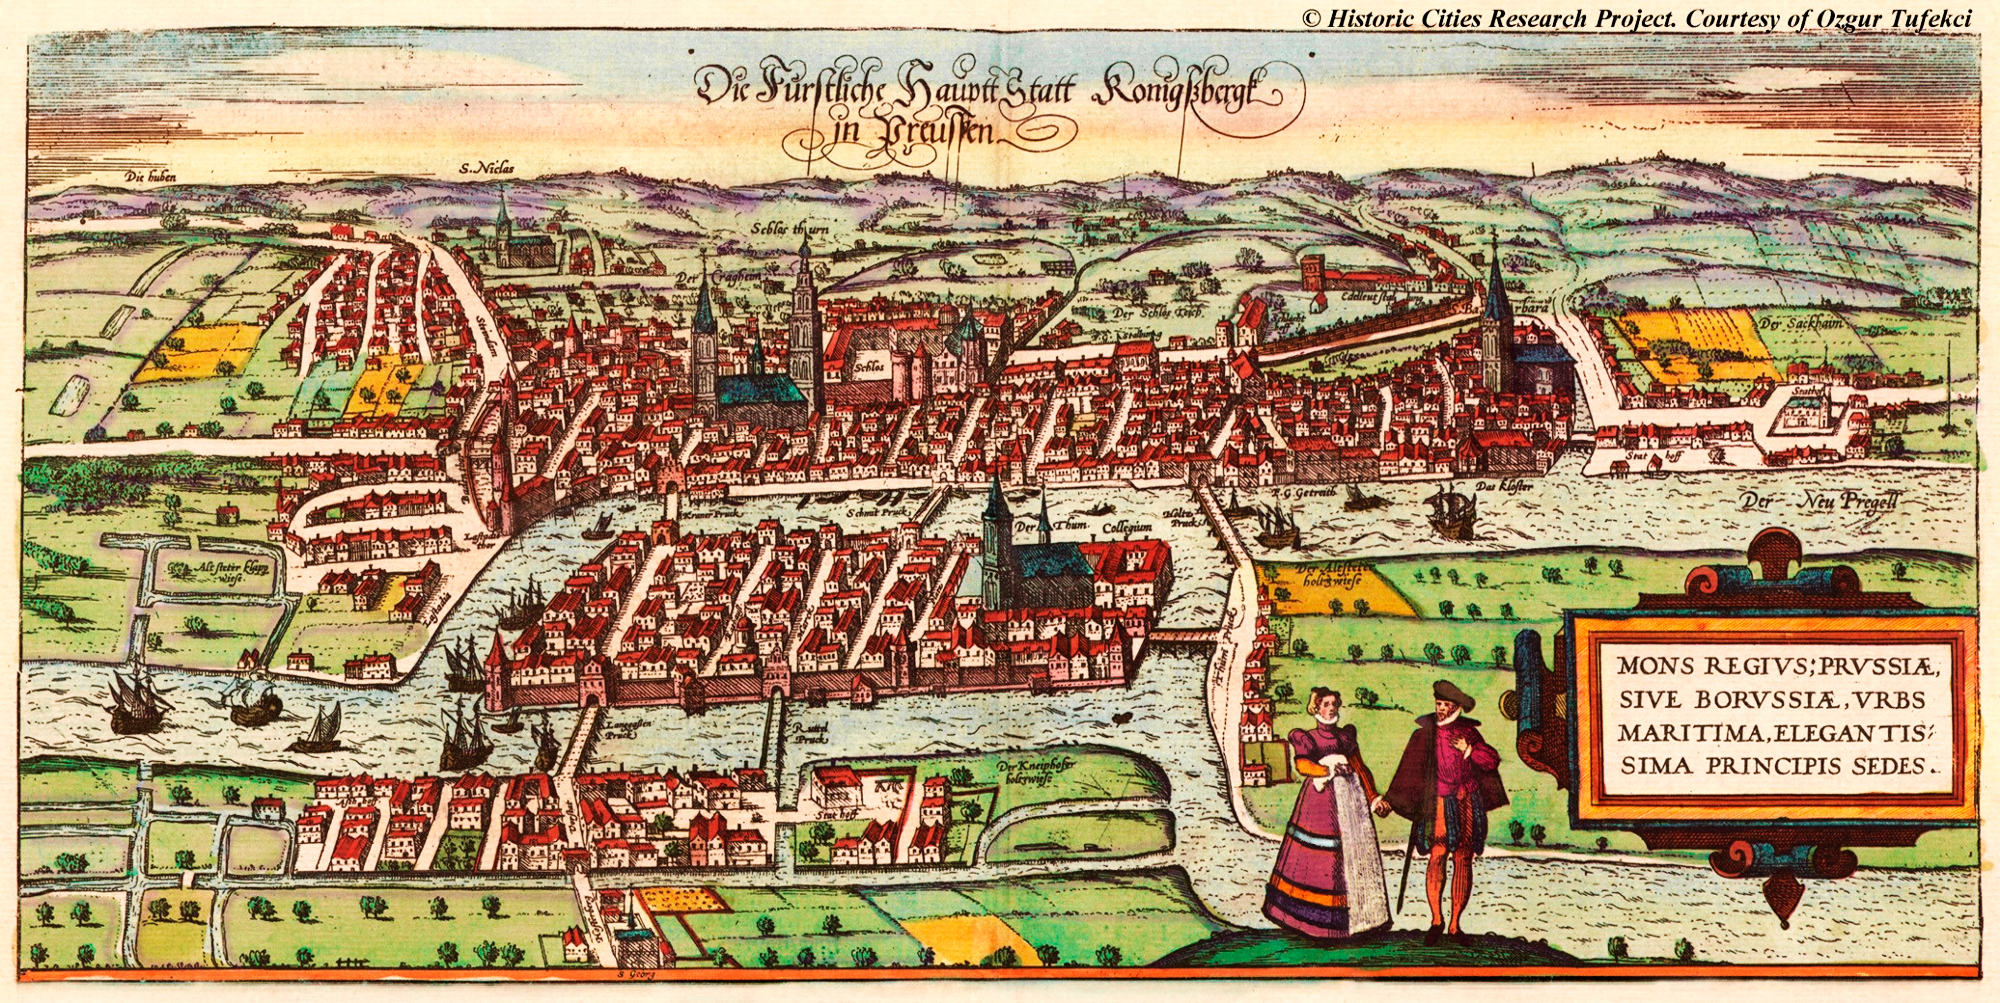
\includegraphics[scale=0.12]{images/konisberg_hc.png}
        \end{figure}
        
    \end{frame}
    
    
    \begin{frame}\frametitle{Los puentes de Könisberg - versión 2}
        \begin{figure}
            \includegraphics[scale=0.23]{images/konisberg2.jpg}
        \end{figure}
    \end{frame}
    
    \begin{frame}\frametitle{Los puentes de Könisberg - versión 3}
        \begin{figure}
            \includegraphics[scale=0.18]{images/konisberg3.jpg}
        \end{figure}
        \pause
        Ahora el problema se reduce a encontrar una caminata  que use cada arista (o puente) una y solo una vez.
    \end{frame}
    
    \begin{frame}
        \begin{observacion}
            $\delta(A)=5$, $\delta(B)=3$, $\delta(C)=3$, $\delta(D)=3$.
        \end{observacion}\pause
        
        \vskip .5cm
        
        Euler, abstrayéndose del problema concreto, razonó de la siguiente manera:\pause
        
        \vskip .5cm 
        \begin{itemize}
            \item Supongamos que el vértice de partida es $x$ y  el de llegada es $y$. Todos los demás los llamo vértices intermedios.\pause
            \item En un vértice intermedio cada vez que entro por un puente salgo por otro. Eso  me ``aporta''  2 a la valencia.\pause
            \item Terminado el proceso usé todos los puentes, por lo tanto  en cada vértice intermedio la cantidad de entradas más la cantidad de salidas es la valencia. Como la cantidad de entradas es igual a la cantidad de salidas, la valencia en los vértices intermedios es par.
            
        \end{itemize}
        
        
    \end{frame}
    
    \begin{frame}
        \textbf{Concluyendo}
        \vskip .3cm
        \begin{itemize}
            \item Si hay una caminata que pasa por cada puente una y solo una vez,  la cantidad de vértices con valencia impar es a lo sumo 2. \pause
            \item Como todos los vértices en el problema tienen valencia impar, el problema no tiene solución. 
        \end{itemize}\pause
        \vskip .3cm
        Como veremos más adelante el problema de los puentes de Könisberg puede ser generalizado y también vale la recíproca.\pause
        \vskip .5cm
        \textbf{Cita:}  Euler, Leonhard (1736). \href{http://math.dartmouth.edu/\~euler/docs/originals/E053.pdf}{Solutio problematis ad geometriam situs pertinentis}. Comment. Acad. Sci. U. Petrop 8, 128-40 (en latín)
        
    \end{frame}
    
    \begin{frame}
        \begin{ejemplo} ¿Es posible recorrer el siguiente gráfo con una caminata que pase por cada vértice una sola vez y volver al de partida? ¿Es posible hacer una caminata  que pasa por cada arista una sola vez?
            \begin{figure}[h]
                \begin{center}
                    \begin{tikzpicture}[scale=1]
                        %\SetVertexSimple[Shape=circle,FillColor=white]
                        \def\rvar{1.2}
                        \Vertex[x=0.00, y=-2.00]{$u$}
                        \Vertex[x=\rvar*1.90, y=-0.62]{$t$}
                        \Vertex[x=\rvar*1.18, y=1.62]{$q$}
                        \Vertex[x=-1.18*\rvar, y=1.62]{$p$}
                        \Vertex[x=-1.90*\rvar, y=-0.62]{$r$}
                        \Vertex[x=0, y=0]{$s$}
                        \Edges($u$,$t$,$q$,$p$,$r$,$u$,$s$,$t$,$r$,$s$,$q$,$r$,$p$,$t$,$s$,$u$,$s$,$p$)
                    \end{tikzpicture}
                \end{center}
            \end{figure}
            
        \end{ejemplo}
    \end{frame}
    
    \begin{frame}
        \begin{solucion}\pause
            Para la primera pregunta una posibilidad es el ciclo $p,q,t,s,u,r,p$.\pause
            
            \vskip .5cm
            
            La segunda pregunta tiene respuesta negativa:\pause
            
            Las valencias son 
            $$\delta(p) = 4,\quad\delta(q) = 4,\quad\delta(s) = 5,\quad\delta(r) = 5,\quad\delta(u) = 3,\quad\delta(t) = 5.$$\pause
            
            Como en los puentes de Königsberg,  al haber más de $2$ vértices de valencia impar, no es posible recorrer todas las aristas una sola vez.
            
            \qed
            
            
            
        \end{solucion}
    \end{frame}
    
        
    \begin{frame}
        \begin{definicion}
            Un {\em ciclo hamiltoniano} en un grafo $G$ es un ciclo que contiene a todos los vértices del grafo.\pause
            \vskip .2cm
            Una {\em caminata euleriana} en un grafo $G$ es un caminata que usa todas las aristas de $G$ exactamente  una vez o,  equivalentemente, un recorrido que utiliza todas las aristas.  \pause
            \vskip .2cm
            Una caminata euleriana que comienza y termina en un mismo vértice se llama también {\em circuito euleriano}.
        \end{definicion}
        
        \vskip .2cm
        
        \begin{teorema}  Un grafo conexo con más de un vértice tiene un circuito euleriano si y sólo si todos los vértices tienen grado par. Un grafo conexo con más de un vértice posee caminatas eulerianas de $v$ a $w$, con $v \not= w$ si y sólo si $v$ y $w$ son los únicos vértices de grado impar.
        \end{teorema}
    \end{frame}

    \begin{frame}
    

        C. Hierholzer (1840-1871) mostró, poco antes de su muerte, un algoritmo fácilmente implementable para encontrar un circuito euleriano  para cualquier grafo  con vértices de grado  par. \pause
        
        \vskip .6cm
        
        El  mismo algoritmo sirve para grafos con dos vértices de grado impar.
        
        \vskip .6cm\pause
        
        Para explicar el algoritmo de Hierholzer nos es útil la siguiente
        
        \vskip .4cm
        
        \begin{definicion}
            Un \textit{recorrido maximal}  es un recorrido que respetando la condición de no repetir aristas no es posible continuarlo.  
        \end{definicion}

        \vskip .2cm

        \vskip .6cm\pause
    \end{frame}
        
    \begin{frame}\frametitle{Algoritmo de Hierholzer: idea clave}\pause
        
        La idea clave del algoritmo de Hierholzer  es la siguiente:  en un grafo de valencias pares (conexo o no conexo) todo recorrido maximal termina en el vértice original.

        \vskip .4cm\pause

        \begin{itemize}
            \item Sea $x$ un vértice del grafo  que será donde comenzará la caminata.
            \item Cada vez que ingreso y salgo de un vértice $v$ ``consumo'' $2$  aristas y  me quedan $2$ aristas menos para utilizar.\pause
            \item Como $\delta(v)$  es par,  si $v\ne x$ cada vez que ingraso y salgo  de $v$ me queda un un número para de aristas de ese vértice sin utilizar.\pause
            \item Es decir,  siempre que puedo entrar a un vértice $v \ne x$, puedo salir.\pause
            \item Es  decir, el único vértice al que puedo entrar y quizás no pueda  salir es $x$.\pause
            \item Como el recorrido es maximal,  va a haber algún momento en que no pueda avanzar más y eso solo puede ocurrir cuando estamos en el vértice $x$.
        \end{itemize}

    \end{frame}

    \begin{frame}
        \frametitle{Algoritmo de Hierholzer: idea de la demostración (1)}\pause
        
        
        Algoritmo  de Hierholzer (grafo con todas valencias pares):\pause
        \vskip .4cm
        \begin{enumerate}
            \item \textbf{Paso 1.} Elija cualquier vértice  inicial $v$ y haga un recorrido  maximal.\pause
            \vskip .2cm
            (recorrido cerrado, puede no cubrir todas las aristas).\pause
            \vskip .4cm
            \item \textbf{Paso iterativo} \pause
            \begin{enumerate}\pause
                \item[\textit{i)}] Mientras exista un vértice $u$ en la caminata ya realizada, pero que tenga aristas que no formen parte de la caminata, inicie otro recorrido maximal (será de $u$ a $u$) siguiendo las aristas no utilizadas.\pause
                \item[\textit{ii)}] Inserte esta  caminata a la caminata  anterior en $u$  para formar una caminata nueva (más larga).\pause
                \item[\textit{iii)}] Si no cubrió todas las aristas vuelva a \textit{i)}.
            \end{enumerate} 
            
        \end{enumerate}
    
    \end{frame}
    
    \begin{frame}\frametitle{Algoritmo de Hierholzer: idea de la demostración (2)}

        En  el paso iterativo el subgrafo que obtenemos luego de quitar las aristas recorridas es par. Esto nos permite hacer caminatas cerradas  por aristas no utilizadas desde cada vértice con aristas no utilizadas.\pause
        \vskip .6cm

        
            El caso de un grafo donde todas las valencias son pares excepto $2$ se puede reducir al anterior: si deseamos una caminata euleriana que empiece por $v$ y termine en $w$.\pause
        \begin{itemize}
            \item Comenzamos en $v$ y haga una caminata  que no repita aristas hasta que se detenga. \pause
            \item Elimine la aristas utilizadas. El grafo que queda es par y  ahí utilizamos el algoritmo para ese caso. 
        \end{itemize}
        
        \qed
        
    \end{frame}
    
    
    
    \begin{frame}
        \begin{ejemplo}
            Encontremos un circuito euleriano del siguiente grafo. 
            \vskip .4cm
            \begin{figure}[ht]
                \begin{center}
                    \begin{tikzpicture}[scale=1]
                    %\SetVertexSimple[Shape=circle,FillColor=white]
                    \def\rvar{1.2}
                    \Vertex[x=0.00, y=-2.00, L=$u$]{$u$} % 3
                    \Vertex[x=\rvar*1.90, y=-0.62, L=$t$]{$t$} % 2
                    \Vertex[x=\rvar*1.18, y=1.62, L=$q$]{$q$} % 1
                    \Vertex[x=-1.18*\rvar, y=1.62, L=$p$]{$p$} % 0
                    \Vertex[x=-1.90*\rvar, y=-0.62, L=$r$]{$r$} % 4
                    \Vertex[x=0, y=0, L=$s$]{$s$} % 5
                    \Edges($u$,$t$,$q$,$p$)
                    \Edges($r$,$u$)
                    \Edges($s$,$t$)
                    \Edges($r$,$s$,$q$,$r$)
                    \Edges($p$,$t$,$s$)
                    \Edges($s$,$p$,$r$)
                    \end{tikzpicture}
                    \end{center}
            \end{figure}
            
        \end{ejemplo}
    \end{frame}
    
    \begin{frame}
        \begin{solucion}
            Debemos primero observar que  debe existir un circuito euleriano, pues $\delta(p)=4$, $\delta(q)=4$, $\delta(r)=4$, $\delta(s)=4$, $\delta(t)=4$, y $\delta(u)=2$,  es decir todos los vértices tienen grado par. \pause
            \vskip .2cm
            
            Apliquemos el algoritmo de Hierholzer partiendo  desde $u$. Una caminata posible con origen en $u$ y que vuelva a $u$ es $$u, r, p, q, s, t, u.$$


            Ahora elijamos $q$ que es un vértice que pertenece a la caminata pero que tiene aristas que no son parte de la caminata. Una caminata que no toca aristas usadas y  que parte de $q$ y regresa a $q$ es $q,t,p,s,r,q$.  \pause

            Insertamos en $q$  esta caminata  a la caminata anterior y obtenemos:
            $$u, r, p, \underline{q,t,p,s,r,q}, s, t, u.$$
            (Subrayada la caminata insertada).

            \qed
        \end{solucion}
    \end{frame}
    

    \begin{frame}[fragile]\frametitle{Recorrido maximal}
Mostramos en pseudocódigo el algoritmo de recorrido maximal. 

\begin{verbatim}
def r_max(L, v_ini): 
    # pre: L grafo, v_ini vértice de L
    # post: recorrido maximal que comienza en v_ini
    sub_caminata = [v_ini]  # sub caminata
    p0 = v_ini
    while len(L.adyacentes(p0)) > 0:  
        p1 = L.adyacentes(p0)[0] # p1 primer adyacente a p0 
        sub_caminata.append(p1) # agrega p1 a caminata
        L.quitar_arista((p0,p1)) # quita arista {p0, p1}
        p0 = p1 
    return sub_caminata
\end{verbatim}
\end{frame}

\begin{frame}[fragile]
    \frametitle{Algoritmo de Hierholzer}
    Mostramos en pseudocódigo el algoritmo de Hierholzer
    
\begin{verbatim}
    # pre: G grafo admisible
    # post: cuando termina 'c' es una caminata
    #       o circuito euleriano que empieza en 0.
    libres = G.copiar() # sub grafo de aristas no utilizadas
    c = r_max(libres, v_ini) # recorrido maximal
    while len(libres.aristas()) > 0: 
        for v in libres.vertices(): 
            if len(libres.adyacentes(v)) > 0 and v in c:
                pos = cam.index(v) 
                c  =  c[:pos] + r_max(libres, v) + c[pos+1:]
\end{verbatim}

\end{frame}

\end{document}

